\documentclass[10pt,a4paper]{article}
\usepackage[margin=2cm]{geometry}
\usepackage{fancyvrb,booktabs,amsmath,amssymb,enumitem,tikz}
\fvset{fontsize=\scriptsize,frame=single}
\title{Lab Report -- Neural Models: Learning, Depth, Activations, Output Layers}
\author{Apurva Verma}
\date{}
\begin{document}
\maketitle

\section*{Task 1: Problem specification}
$\mathcal X=\{0,1\}^2$, $\mathcal Y=\{0,1\}$. Labelled examples: $(0,0)\!\to\!0$, $(0,1)\!\to\!1$, $(1,0)\!\to\!1$, $(1,1)\!\to\!0$ (XOR: warning iff the sensors disagree).

\textbf{Plot:} in the $x_1,x_2$ plane the class-0 points sit at opposite corners $(0,0),(1,1)$ and the class-1 points at the other corners $(0,1),(1,0)$, so the two classes lie on the two diagonals of the unit square.


\begin{center}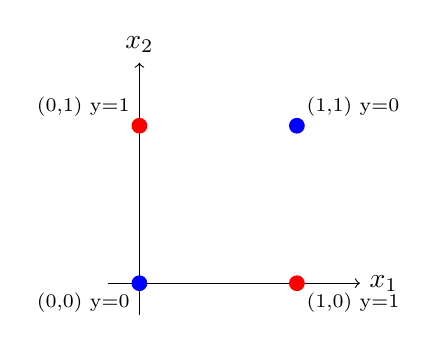
\begin{tikzpicture}[scale=2]
\draw[->] (-0.2,0)--(1.4,0) node[right]{$x_1$}; \draw[->] (0,-0.2)--(0,1.4) node[above]{$x_2$};
\foreach \p in {(0,0),(1,1)} \fill[blue] \p circle(0.05);
\foreach \p in {(0,1),(1,0)} \fill[red] \p circle(0.05);
\node[below left] at (0,0) {\scriptsize (0,0) y=0}; \node[above right] at (1,1) {\scriptsize (1,1) y=0};
\node[above left] at (0,1) {\scriptsize (0,1) y=1}; \node[below right] at (1,0) {\scriptsize (1,0) y=1};
\end{tikzpicture}\end{center}
\textbf{Linear separability:} a line $w_1x_1+w_2x_2+b=0$ would need $b<0$, $w_1+w_2+b<0$ (class 0) and $w_1+b>0$, $w_2+b>0$ (class 1). Adding the last two gives $w_1+w_2+2b>0$, but adding the first two gives $w_1+w_2+2b<0$: a contradiction, so no straight boundary works.

\textbf{Prediction:} a single affine map plus sigmoid can do no better than predicting $\approx0.5$ for every input (loss $\approx\ln2$), getting at most 3 of 4 correct.

\section*{Task 2: Model design and validation criteria}
Design: 2 inputs $\to$ 2 hidden units (tanh; sigmoid and ReLU tried later) $\to$ 1 output logit; sigmoid output, binary cross-entropy (implemented as \texttt{BCEWithLogitsLoss}), Adam, full batch.

\begin{enumerate}[leftmargin=*]
\item \textbf{Why nonlinearity:} affine layers collapse to one affine map, which is a linear classifier and cannot represent XOR. The hidden nonlinearity lets the network re-represent the inputs in a space where the classes become linearly separable. Depth alone does not help; nonlinearity does. XOR tests exactly this claim about representation with four points.
\item \textbf{Why sigmoid + BCE:} the target is one yes/no answer; sigmoid maps the logit to a probability in $(0,1)$, BCE is the negative log-likelihood of a Bernoulli label, and the logit gradient is simply $p-y$ (no saturation-induced vanishing from the loss).
\item \textbf{Success evidence:} (a) final loss far below $\ln2\approx0.693$; (b) all four thresholded predictions correct; (c) first-layer gradient nonzero at an early step and finite-difference check agrees with autograd; (d) repeated-run behaviour over several seeds; (e) zero-init control fails, showing the learning is not trivial.
\end{enumerate}
\textit{Hidden units get no targets:} what each computes is determined only by the output-layer loss propagated backwards through the chain rule; backprop supplies each hidden unit a learning signal $\partial L/\partial h$.

\section*{Task 3: LLM prompts and generated code}
The prompts below were used with LLM assistance to produce the code, which was inspected and run. Forward pass: \texttt{forward()}; scalar loss: \texttt{criterion(logits,y)}; reverse-mode AD: \texttt{loss.backward()}; parameter update: \texttt{optimizer.step()}.

\textbf{Two changes made after the first run of the generated code:} (1) a progress print of the loss every 500 steps, to see the loss decreasing rather than only the final number; (2) an \texttt{assert torch.isfinite(loss)} guard inside the training loop to catch NaN/inf immediately. Neither changes the architecture, data, loss or optimiser. The logged losses for seed 0 were 0.7152 (step 0), 0.00194 (500), 0.00064 (1000), 0.00032 (1500), 0.00019 (2000), 0.00012 (2500).

\subsection*{Prompt 1 (Task 3)}
\begin{Verbatim}
Generate minimal PyTorch code for the following model and dataset. Do not change the architecture or task.

Dataset (XOR, sensor-disagreement warning), all 4 examples, full batch:
x = [[0,0],[0,1],[1,0],[1,1]], y = [0,1,1,0]

Model: 2 inputs -> 2 hidden units (tanh activation) -> 1 output logit.
Use nn.Linear layers with PyTorch's default random initialisation.
Output: a single logit, trained with BCEWithLogitsLoss (mean reduction); apply sigmoid only to report probabilities.
Optimiser: Adam, lr=0.05, full-batch training for 3000 CPU steps.
Set torch.manual_seed(0) for reproducibility.

After training, report: the initial loss, the final loss, all four probabilities, the labels thresholded at 0.5, whether all 4 are correct, and the gradient tensor of the first-layer weight (layer1.weight.grad) after a forward pass and backward().
Add brief comments marking where the forward pass happens, where the scalar loss is formed, where backward() (reverse-mode AD) is invoked, and where optimizer.step() updates the parameters.
Save as task3_xor.py and run it. Explain each test in one sentence.
\end{Verbatim}
\subsection*{Prompt 2 (Task 4 A--C)}
\begin{Verbatim}
Using task3_xor.py without changing the architecture or task, create task4_diagnostics.py that does the following:

Part A: repeat the basic learning check for seeds 0 to 4 and report the initial loss, final loss and 4/4 correctness for each seed.
Part B: for one forward+backward pass at initialisation, print layer1.weight.grad. Verify it against a finite-difference estimate of dL/dW1 (eps=1e-4). Also show numerically that the mean-loss gradient equals the average of the four per-example gradients.
Part C: copy the experiment but set ALL weights and biases to zero before training (same architecture). Train and print the two rows of the hidden-layer weight matrix at steps 0, 1, 2, 5, 10, 100 and at the final step, and report whether the rows stay identical. Also report the final loss and predictions.
Run it and show the output.
\end{Verbatim}
\subsection*{Prompt 3 (Task 4 D)}
\begin{Verbatim}
Create task4_activations.py. Train the same random-initialised 2-2-1 XOR network three times, changing ONLY the hidden activation: sigmoid, tanh, ReLU. Keep the same seed, optimiser (Adam lr=0.05), 3000 steps and BCEWithLogitsLoss.
For each run, record: the final loss, whether all 4 examples are classified correctly, and the Euclidean (L2) norm of the first-layer weight gradient at step 1 (an early step).
Also print the hidden pre-activations and activations at the end, so we can tell sigmoid saturation apart from dead ReLU units.
Because 4 data points and 1 seed are fragile, also repeat over seeds 0 to 9 and report how many of the 10 runs succeed for each activation.
Print a result table with columns: Hidden activation | Final loss | 4/4 correct? | Early ||grad W1||_2.
\end{Verbatim}
\subsection*{Prompt 4 (Task 5)}
\begin{Verbatim}
Modify ONLY the output/loss portion of task3_xor.py to make task5_multiclass.py:
Classes: 0 = (0,0) both inactive, 1 = (0,1) or (1,0) disagree, 2 = (1,1) both active.
Keep the 2-unit tanh hidden layer. Replace the output with nn.Linear(2, 3) producing 3 logits, trained with nn.CrossEntropyLoss.
Before training, print the shape of the final weight matrix and the logits shape per example.
After training, print the softmax probability vectors for all four inputs and the predicted classes, and verify that one probability vector sums to about 1.
Verify numerically that the gradient of the loss with respect to the logits equals (p - y_onehot)/N.
Optional diagnostic: add 100 to all three logits and show the softmax output is unchanged; then show that a naive exp() overflows with a large shift (e.g. +1000) while the max-subtracted version does not.
\end{Verbatim}

\section*{Task 4: Results}
\subsection*{Part A (basic learning check)}
Seed 0: initial loss 0.7152, final 0.000083; probabilities $[5.9\text{e-}5,\,0.99990,\,0.99988,\,5.1\text{e-}5]$; labels $[0,1,1,0]$; 4/4 correct. Seeds 0--4: seeds 0, 2, 3, 4 succeed (final loss $\approx10^{-4}$); seed 1 stalls at loss 0.3466 with 1 example wrong (a poor local minimum), so success is not guaranteed for a 2-unit hidden layer.

\subsection*{Part B (backprop check)}
\texttt{layer1.weight.grad} is $\partial L/\partial W^{(1)}$, the derivative of the scalar mean loss w.r.t.\ each first-layer weight. At init (seed 0) autograd gives $[[0.0005,0.0006],[-0.0426,-0.0448]]$; central finite differences ($\epsilon=10^{-4}$) give $[[0.0009,0.0009],[-0.0423,-0.0447]]$, max abs difference $3.9\times10^{-4}$ (float32 roundoff). The mean-loss gradient equals the average of the four per-example gradients (verified, \texttt{True}) because differentiation is linear: $\nabla\frac1N\sum_i L_i=\frac1N\sum_i\nabla L_i$.

\subsection*{Part C (zero-initialisation symmetry)}
The two rows of $W^{(1)}$ are identical at steps 0, 1, 2, 5, 10, 100 and 3000 (in fact they stay exactly $[0,0]$). Final loss $0.6931=\ln2$, all probabilities 0.5, not 4/4 correct. Identical hidden units compute the same output and, since the output weights are also identical (zero), receive the same gradient, so every update keeps them identical; symmetry is never broken. (With all-zero weights, tanh gives zero hidden activations, so the output-weight gradient is also zero, and the first-layer gradient is zero because the output weights are zero: the network is also at a saddle point.)

\subsection*{Part D (activation experiment, seed 0, Adam lr 0.05, 3000 steps)}
\begin{center}\begin{tabular}{lcccc}\toprule
Hidden activation & Final loss & 4/4 correct? & Early $\|\nabla_{W^{(1)}}L\|_2$ & Seeds OK (of 10)\\\midrule
Sigmoid & 0.4774 & No & 0.000891 & 4\\
Tanh & 0.000083 & Yes & 0.061785 & 4\\
ReLU & 0.6931 & No & 0.001699 & 3\\\bottomrule\end{tabular}\end{center}
\textbf{Interpretation.} For this single seed, tanh learned XOR while sigmoid and ReLU did not, and the tanh early gradient was much larger ($\sim$70$\times$ sigmoid, $\sim$36$\times$ ReLU). The hidden-layer inspection shows different mechanisms: the sigmoid run ended with large $|$pre-activations$|$ ($\pm$11 to $\pm$25) and activations pinned near 0/1, i.e.\ saturation with tiny derivatives; the ReLU run ended with all pre-activations negative and all activations exactly 0, i.e.\ dead units with zero gradient. However, across seeds 0--9 the success counts are 4/10, 4/10 and 3/10, so with four data points and a 2-unit hidden layer I do not conclude any activation is universally better; the seed-0 difference is largely about initial conditions. Saturation vs.\ dead ReLU is distinguished by pre-activations: large magnitude with activation near 0/1 (sigmoid) versus negative pre-activation with activation exactly 0 (ReLU).

\section*{Task 5: Three-class extension}
Output changed to \texttt{nn.Linear(2,3)} with \texttt{CrossEntropyLoss}. Predictions made beforehand: final weight matrix shape $3\times2$; 3 logits per example; softmax sums to one because $\sum_k e^{z_k}/\sum_j e^{z_j}=1$ by construction; logit gradient $p-y$ because $L=-\log p_y$ and $\partial L/\partial z_k=p_k-\mathbb 1[k=y]$. Confirmed: weight shape $(3,2)$, logits shape $(3,)$. Final loss $3.9\times10^{-5}$; predicted classes $[0,1,1,2]$ match targets. Probabilities:
\begin{Verbatim}
(0,0): [9.9995e-01, 4.8949e-05, 7.3595e-09]
(0,1): [2.3397e-05, 9.9997e-01, 7.4549e-06]
(1,0): [2.3177e-05, 9.9997e-01, 7.0238e-06]
(1,1): [2.7497e-07, 4.5178e-05, 9.9995e-01]
\end{Verbatim}
For input (0,1) the probabilities sum to $1.0$. The gradient w.r.t.\ logits equals $(p-y_{\text{onehot}})/N$ (\texttt{True}; the $1/N$ comes from the mean loss). Adding 100 to all logits leaves softmax unchanged (\texttt{True}), because the common factor $e^{100}$ cancels. A naive \texttt{exp} with $+1000$ overflows to \texttt{nan}; subtracting the max logit first gives the correct result, which is why stable implementations do so.

\section*{Reflection Questions}
\begin{enumerate}[leftmargin=*]
\item Depth is not enough: stacking affine layers is still one affine map. The nonlinear activation is what lets a hidden layer make XOR separable; depth then composes nonlinear features.
\item The loss fell from 0.715 to $8\times10^{-5}$ and all four predictions flipped to the right XOR labels, and the autograd gradient matched finite differences. The gradient therefore pointed in a useful descent direction, not merely a nonzero one. (The zero-init run had nonzero-looking machinery but loss stuck at $\ln2$.)
\item With identical weights, both hidden units compute the same output and get the same gradient, so they remain identical forever; two units act as one and cannot form distinct features. Random init breaks the symmetry.
\item Scientific: sigmoid saturates (derivative $\le0.25$, near 0 when saturated), tanh has derivative up to 1 and is zero-centred, ReLU has derivative 1 when active but exactly 0 when the unit is negative. Engineering observation: early gradient norms were 0.00089 (sigmoid), 0.0618 (tanh), 0.0017 (ReLU) for seed 0, but success rates over 10 seeds were similar (4/4/3), so the gradient size at one step is not a reliable predictor alone.
\item The output activation and loss must match the target type and probabilistic model: sigmoid+BCE for one Bernoulli label, softmax+cross-entropy for one-of-$K$. Mismatches (e.g.\ softmax with BCE, or MSE on logits) give wrong likelihoods and worse gradients; the matched pair gives the clean $p-y$ logit gradient.
\item Productivity: the LLM produced the boilerplate and tests (finite differences, per-example gradients, stability demo) quickly. Human verification was essential for checking that the code implements the specified 2--2--1 experiment, for noticing seed 1 fails and that the 10-seed counts contradict a naive ``tanh is best'' reading of one run, and for interpreting the finite-difference gap as float32 roundoff.
\item Keep: loss/prediction checks, gradient-norm monitoring, NaN/overflow checks, symmetry-breaking init, multi-seed repeats, cheap per-layer activation statistics, and spot-checks of a few gradient entries. Too expensive at scale: exhaustive finite-difference gradient checks (cost $\propto$ number of parameters), and running many seeds of full training.
\end{enumerate}

\section*{Code}
\subsection*{task3\_xor.py}\VerbatimInput{task3_xor.py}
\subsection*{task4\_diagnostics.py}\VerbatimInput{task4_diagnostics.py}
\subsection*{task4\_activations.py}\VerbatimInput{task4_activations.py}
\subsection*{task5\_multiclass.py}\VerbatimInput{task5_multiclass.py}
\end{document}
